
\begin{figure}[htbp]
\centering
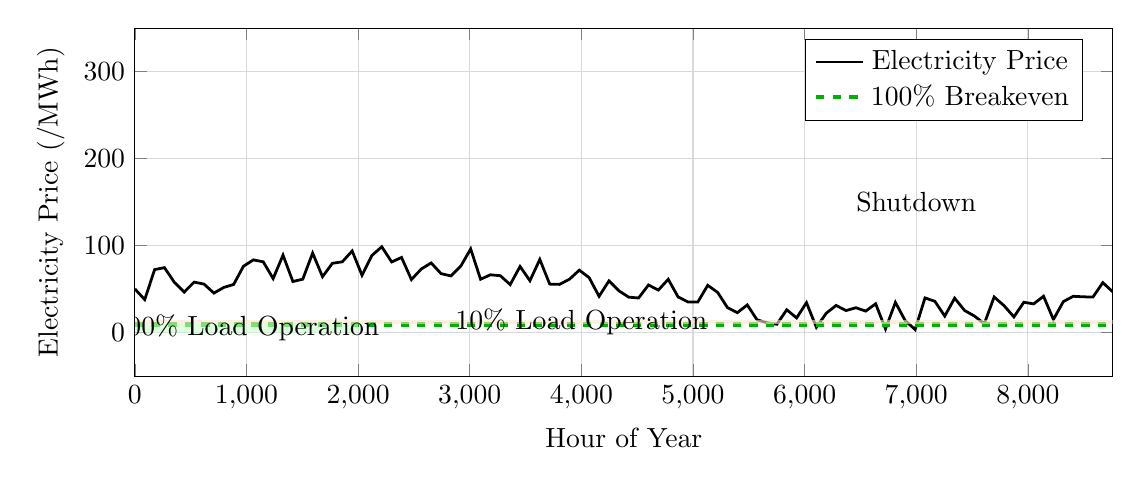
\begin{tikzpicture}
\begin{axis}[
    width=14cm,
    height=6cm,
    xlabel={Hour of Year},
    ylabel={Electricity Price (\euro/MWh)},
    xmin=0,
    xmax=8760,
    ymin=-50,
    ymax=350,
    grid=major,
    grid style={gray!30},
    legend pos=north east,
    every axis plot/.append style={line width=1pt}
]

% Simplified price profile (representative data)
\addplot[
    color=black,
    mark=none,
    samples=100,
    domain=0:8760,
] {50 + 30*sin(deg(x/1460)) + 20*rand};

% Breakeven lines
\addplot[
    color=green!70!black,
    dashed,
    line width=1.5pt,
    domain=0:8760,
] {9.42};

% Operation zones (simplified)
\fill[green!20, opacity=0.6] (axis cs:0,0) rectangle (axis cs:2000,9.42);
\fill[orange!20, opacity=0.6] (axis cs:0,9.42) rectangle (axis cs:8760,15);

\node at (axis cs:1000,5) {100\% Load Operation};
\node at (axis cs:4000,12) {10\% Load Operation};
\node at (axis cs:7000,150) {Shutdown};

\legend{Electricity Price, 100\% Breakeven}

\end{axis}
\end{tikzpicture}
\caption{Operational strategy based on electricity price thresholds}
\label{fig:operational-profile}
\end{figure}
